\documentclass{article}
\usepackage{fullpage}
\usepackage{graphicx}
\usepackage{amsmath}

\title{Shor}
\author{Jacques Carette \and Gerardo Ortiz \and Amr Sabry}

\begin{document}
\maketitle

\newcommand{\st}[5]{\ensuremath{| #1, #2, #3, #4, #5 \rangle}}
\newcommand{\ket}[1]{\ensuremath{| #1 \rangle}}

%%%%%%%%%%%%%%%%%%%%%%%%%%%%%%%%%%%%%%%%%%%%%%%%%%%%%%%%%%%%%%%%%%%%%%%%%%%%%%%%%%
\section{Claims}

\paragraph*{Claim I.}
An efficient generate-and-test algorithm of expmod would allow an
efficient classical implementation of Shor's algorithm.

\paragraph*{Claim II.}
It is possible to realize an efficient generate-and-test algorithm for
expmod by using partial evaluation and reverse execution.

%%%%%%%%%%%%%%%%%%%%%%%%%%%%%%%%%%%%%%%%%%%%%%%%%%%%%%%%%%%%%%%%%%%%%%%%%%%%%%%%%%
\section{Purity Analysis of Shor's Algorithm}

No entanglement; conjecture that it is implementable using classical waves. 

Consider the expmod block of Shor's algorithm. Let the state on the
right be $\Sigma_{x~s.t.~f(x) = r} \ket{x,r}$ and let's do the
retrocausal propagation. What is the state at different points going
backwards towards the initial state? How much entanglement is
generated. It is probably the case that the amount of entanglement
generated is related to the complexity of the boolean formulae we
generate. Indeed running backwards with an unknown state and
collecting constraints along the way must be identical to the quantum
propagation in this particular example.

%%%%%%%%%%%%%%%%%%%%%%%%%%%%%%%%%%%%%%%%%%%%%%%%%%%%%%%%%%%%%%%%%%%%%%%%%%%%%%%%%%
\section{Generate-and-Test Shor}

Here is a way of writing a classical algorithm that mimics the
structure of Shor's algorithm:

\begin{verbatim}
generateAndTest :: (Integer -> Integer) -> Integer -> Integer -> [Integer]
generateAndTest f range obs =
  map fst [ (x, f x) | x <- [0..range], f x == obs]

shor :: Integer -> IO (Integer,Integer)
shor n = 
  do x <- randomRIO (2, n - 1)
     let f r = powModInteger x r n                       
     test <- randomRIO (0, (n * n))
     let (a : b : _) = generateAndTest f (n * n) (f test)
     let period = b - a                                  
     let p1 = x ^ (period `div` 2) - 1                   
     let p2 = x ^ (period `div` 2) + 1                   
     return (gcd n p1, gcd n p2)                         
\end{verbatim}

All computations in \verb|shor| are trivial except the call to
\verb|generateAndTest|. If we had an efficient way of implementing
this functionality we would have an efficient factoring algorithm.     

%%%%%%%%%%%%%%%%%%%%%%%%%%%%%%%%%%%%%%%%%%%%%%%%%%%%%%%%%%%%%%%%%%%%%%%%%%%%%%%%%%
\section{Example I: Adder}

We illustrate the idea of partial reverse evaluation using a small example.

\begin{center}
  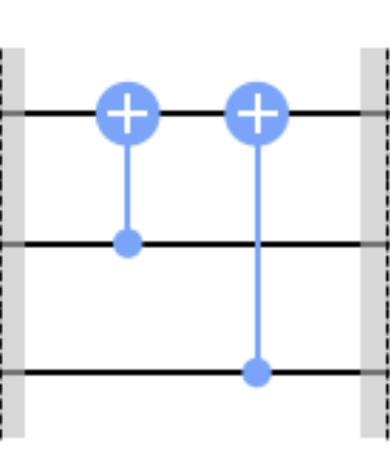
\includegraphics[scale=0.5]{bac-adder.png}
\end{center}

Say we fix the input for the top wire to be 0 and the output to be
1. We can reason as follows:

\begin{itemize}
\item Start backwards evaluation with the state \ket{1,x,y}.
\item If $y=0$, the top wire remains 1; and if $y=1$ the top wire is
  negated to 0. In otherwise, the top wire has the value
  $\overline{y}$ where the overline is boolean negation. The state is
  now \ket{\overline{y},x,y}.
\item If $x=0$, the top wire remains as $\overline{y}$ and if $x=1$
  the top wire becomes $y$. A little of algebra shows that the top
  wire will have the value $\overline{x \oplus y}$ where $\oplus$ is
  xor. The final state is \ket{\overline{x \oplus y}, x, y}.
\item If the boundary condition fixes the top input to be 0, then we
  want $\overline{x \oplus y}$ to be 0 which happens when $x \neq y$.  
\end{itemize}
So we propagated some information from the output to gain some
information about the input and did this efficiently.

%%%%%%%%%%%%%%%%%%%%%%%%%%%%%%%%%%%%%%%%%%%%%%%%%%%%%%%%%%%%%%%%%%%%%%%%%%%%%%%%%%
\section{Example II: IBM Shor 21}

The following figure is from the IBM experiment factoring 21.

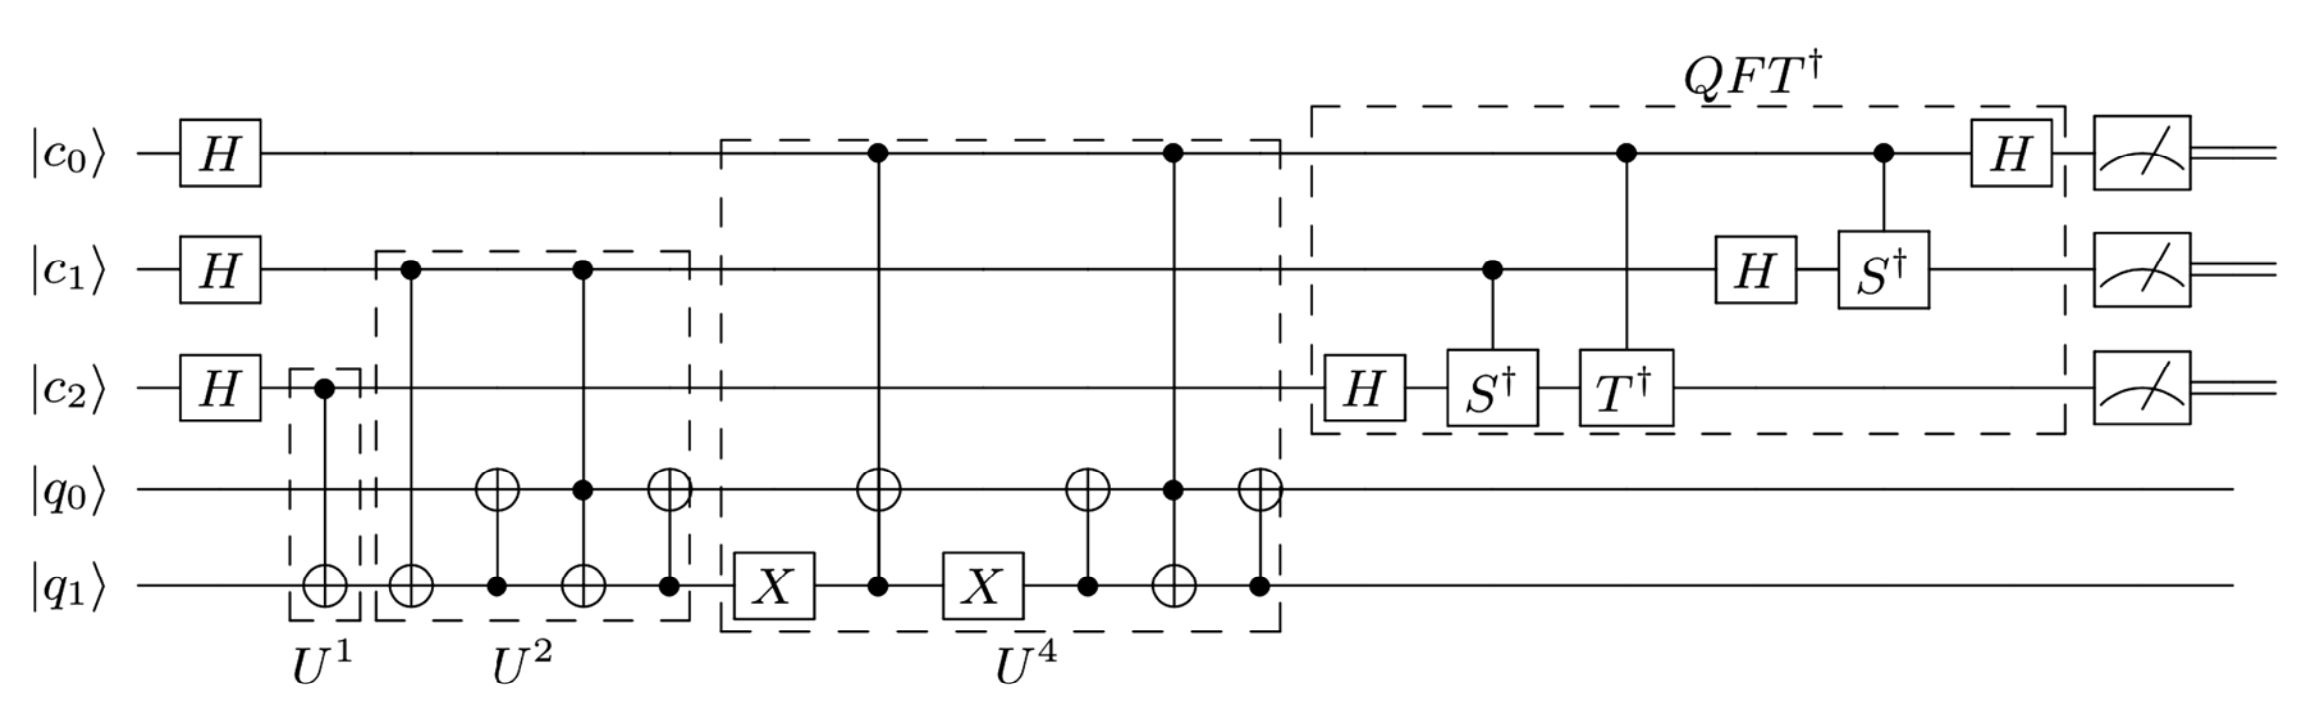
\includegraphics[scale=0.4]{ibmcircuit.png}

Ignore the Hadamard gates at the beginning and the QFT circuit at the
end. Let's start evaluating backwards starting from the partially
known state \st{a}{b}{c}{0}{1}

\begin{itemize}
\item After the first \textsf{cnot} gate (from the end), the states
  becomes \st{a}{b}{c}{1}{1}.
\item Next we have a Toffoli gate with one control wire known to be 1
  and the other is the unknown value~$a$. The resulting state
  is \st{a}{b}{c}{1}{\overline{a}} where the overline is boolean negation.
\item Next we have a \textsf{cnot} gate with the control wire
  $\overline{a}$. The result state is \st{a}{b}{c}{a}{\overline{a}}.
\item Then we have an \textsf{X} gate. The resulting state is
  \st{a}{b}{c}{a}{a}.
\item Then we have another \textsf{Toffoli} gate. The resulting state is
   \st{a}{b}{c}{0}{a}.
\item Then we have an \textsf{X} gate. The resulting state is
  \st{a}{b}{c}{0}{\overline{a}}.
\item Then we have a \textsf{cnot} gate. The result state is
    \st{a}{b}{c}{\overline{a}}{\overline{a}}.
\item Then we have a \textsf{Toffoli} gate. The resulting state is
   \st{a}{b}{c}{\overline{a}}{\overline{a}\overline{b}}.
\item Then we have a \textsf{cnot} gate. The result state is
      \st{a}{b}{c}{\overline{a}b}{\overline{a}\overline{b}}.
\item Then we have another \textsf{cnot} gate. The result state is
      \st{a}{b}{c}{\overline{a}b}{b+\overline{a}}.
\item After the last \textsf{cnot}, the final state is
      \st{a}{b}{c}{\overline{a}b}{\textsf{cx}(c,b+\overline{a})}.
\end{itemize}

Now if the initial state was supposed to be \st{a}{b}{c}{1}{1}, then we
can reason that all of $a$, $b$, and $c$ must be 0.

%%%%%%%%%%%%%%%%%%%%%%%%%%%%%%%%%%%%%%%%%%%%%%%%%%%%%%%%%%%%%%%%%%%%%%%%%%%%%%%%%%
\section{Example III: Applying the Idea to Shor (Outline)}

We want to factor 15:
\begin{itemize}
\item $N = 15$, $N^2 = 225$, so the number of qubits in the first
  register $q=8$; and the second register needs $n=4$ qubits;
\item Choose $a=8$; then $f(x) = 8^x \mod{15}$
\item The main body of the algorithm needs an efficient circuit implementing:
  \[
  U_f : \ket{x}_8\ket{0}_4 \rightarrow \ket{x}_8\ket{f(x)}_4
  \]
\item Choose a random input, say 1, compute $f(1) = 8$ and use that
  value 8 as the starting point for backwards evaluation. In other
  words, we want to run this circuit with the following partially
  known state backwards:
  \[
  \ket{x}_8\ket{8}_4
  \]
  We will match the result with $\ket{x}_8\ket{0}_4$ to derive
  constraints on $x$. We expect to see the following
  $\ket{\_,\_,\_,\_,\_,\_,0,1}$ indicating that all the values $x$ that match
  this output differ by 4.
\end{itemize}

%% *Shor> shor 15
%% 	x = 8
%% 	test = 5; obs = 8
%% 	a = 1, b = 5, period = 4
%% (3,5)

%%%%%%%%%%%%%%%%%%%%%%%%%%%%%%%%%%%%%%%%%%%%%%%%%%%%%%%%%%%%%%%%%%%%%%%%%%%%%%%%%%
\section{Partial Evaluation}

It is critical to write programs at an abstraction level that has a
rich equational theory of fine grained transformations. If
multiplication is a primitive operation then we need domain knowledge
to develop such fine grained transformations; if it expressed in
binary it is too low level. We use numbers $\mod{N}$ as our
representation and write addition, multiplication, and exponentiation
from scratch.

%% https://en.wikipedia.org/wiki/Tonelli–Shanks_algorithm

Instead of starting with exponentiation directly, we start with the
following problem that is equivalent to integer factorization. Given
$n$, $n$, and some $r$ such that $r^2 \equiv n (\mod{N})$ find
$r$. For general $N$ this is equivalent to integer
factorization. Might be an easier function to write and partial
evaluate.

Ex. \verb|f(x,y) = x * (y+1)|; I know y=1. I can conclude the output is even!

%%%%%%%%%%%%%%%%%%%%%%%%%%%%%%%%%%%%%%%%%%%%%%%%%%%%%%%%%%%%%%%%%%%%%%%%%%%%%%%%%%
\section{Gottesman-Knill}

Our symbolic evaluation with ANF will generate linear equations (no
more than one variable in each xor clause). That is known to be
efficient. But we need to deal with phase gates first. 

%%%%%%%%%%%%%%%%%%%%%%%%%%%%%%%%%%%%%%%%%%%%%%%%%%%%%%%%%%%%%%%%%%%%%%%%%%%%%%%%%%

\appendix

\section{Code for PE of Shor (works for 15)}

\begin{verbatim}
{-# LANGUAGE RankNTypes #-}
{-# LANGUAGE MultiWayIf #-}
{-# LANGUAGE TemplateHaskell #-}

module Shor where

import Data.Maybe (catMaybes, maybe, fromJust)
import Data.List (find,union,intersperse)

import qualified Data.Sequence as S
import Data.Sequence (Seq, singleton, viewl, ViewL(..), (><))

import Control.Lens hiding (op,(:<))
import Control.Monad 
import Control.Monad.ST
import Data.STRef

import System.Random
import GHC.Integer.GMP.Internals
  
import Text.Printf (printf)
import Test.QuickCheck hiding ((><))
import Control.Exception.Assert (assert, assertMessage)
import qualified Debug.Trace as Debug

----------------------------------------------------------------------------------------
-- Simple helpers

-- Debug Helpers

debug = True

trace :: String -> a -> a
trace s a = if debug then Debug.trace s a else a

traceM :: Applicative f => String -> f ()
traceM s = if debug then Debug.traceM s else pure ()

-- Numeric computations

fromInt :: Int -> Integer -> [Bool]
fromInt len n = bits ++ replicate (len - length bits) False 
  where bin 0 = []
        bin n = let (q,r) = quotRem n 2 in toEnum (fromInteger r) : bin q
        bits = bin n

toInt :: [Bool] -> Integer
toInt bs = foldr (\ b n -> toInteger (fromEnum b) + 2*n) 0 bs

doublemods :: Integer -> Integer -> [Integer]
doublemods a m = a : doublemods ((2*a) `mod` m) m

sqmods :: Integer -> Integer -> [Integer]
sqmods a m = am : sqmods (am * am) m
  where am = a `mod` m

invmod :: Integer -> Integer -> Integer
invmod x m = loop x m 0 1
  where
    loop 0 1 a _ = a `mod` m
    loop 0 _ _ _ = error "Panic: Inputs not coprime"
    loop x b a u = loop (b `mod` x) x u (a - (u * (b `div` x)))

invsqmods :: Integer -> Integer -> [Integer]
invsqmods a m = invam : invsqmods (am * am) m
  where am = a `mod` m
        invam = a `invmod` m 

----------------------------------------------------------------------------------------
-- Circuits are sequences of generalized Toffoli gates manipulating
-- locations holding static boolean values or dynamic values

--
-- Values with either static or dynamic information
-- ------------------------------------------------

type Literal = (Bool,String)

data Value = Static Bool
           | Symbolic Literal
           | And Literal Literal
           | Or Literal Literal
           | Xor Literal Literal
  deriving Eq

instance Show Value where
  show (Static b) = if b then "1" else "0"
  show (Symbolic (b,s)) = if b then s else ("-" ++ s)
  show (And lit1 lit2) = 
    printf "(%s . %s)" (show (Symbolic lit1)) (show (Symbolic lit2))
  show (Or lit1 lit2) = 
    printf "(%s + %s)" (show (Symbolic lit1)) (show (Symbolic lit2))
  show (Xor lit1 lit2) = 
    printf "(%s # %s)" (show (Symbolic lit1)) (show (Symbolic lit2))

-- Symbolic boolean operations when some values are known

data Formula = NEG Value
             | AND Value Value
             | XOR Value Value

instance Show Formula where
  show (NEG v) = printf "(not %s)" (show v)
  show (AND v1 v2) = printf "(%s . %s)" (show v1) (show v2)
  show (XOR v1 v2) = printf "(%s # %s)" (show v1) (show v2)

extractLiteralsV :: Value -> [String]
extractLiteralsV (Static _) = []
extractLiteralsV (Symbolic (b,s)) = [s]
extractLiteralsV (And (_,s1) (_,s2)) = union [s1] [s2]
extractLiteralsV (Or (_,s1) (_,s2))  = union [s1] [s2]
extractLiteralsV (Xor (_,s1) (_,s2)) = union [s1] [s2] 

extractLiteralsF :: Formula -> [String]
extractLiteralsF (NEG v) = extractLiteralsV v
extractLiteralsF (AND v1 v2) = union (extractLiteralsV v1) (extractLiteralsV v2)
extractLiteralsF (XOR v1 v2) = union (extractLiteralsV v1) (extractLiteralsV v2)

type Env = [(String,Bool)]

makeEnv :: [String] -> [Env]
makeEnv = env
  where baseEnv :: String -> Env
        baseEnv s = [ (s,b) | b <- [False, True] ]

        env :: [String] -> [Env]
        env [] = [[]]
        env (s:ss) = [ t:ts | t <- baseEnv s, ts <- env ss ]

evalValue :: Value -> Env -> Bool
evalValue (Static b) env = b
evalValue (Symbolic (b,s)) env = (not b) /= (fromJust $ lookup s env)
evalValue (And lit1 lit2) env = evalValue (Symbolic lit1) env && evalValue (Symbolic lit2) env
evalValue (Or lit1 lit2)  env = evalValue (Symbolic lit1) env || evalValue (Symbolic lit2) env
evalValue (Xor lit1 lit2) env = evalValue (Symbolic lit1) env /= evalValue (Symbolic lit2) env

evalFormula :: Formula -> Env -> Bool
evalFormula (NEG v) env = evalValue v env
evalFormula (AND v1 v2) env = evalValue v1 env && evalValue v2 env
evalFormula (XOR v1 v2) env = evalValue v1 env /= evalValue v2 env

evalV :: Value -> [String] -> [(Env,Bool)]
evalV v vars = [ (env, evalValue v env) | env <- makeEnv vars ]

evalF :: Formula -> [String] -> [(Env,Bool)]
evalF f vars = [ (env, evalFormula f env) | env <- makeEnv vars ]

generateValues :: [String] -> [Value]
generateValues [] = [Static False, Static True]
generateValues [s] = generateValues [] ++ [Symbolic (False,s) , Symbolic (True,s)] 
generateValues [s1,s2] = foldr union [] [vs1,vs2,ands,ors,xors]
  where vs1 = generateValues [s1]
        vs2 = generateValues [s2]
        pairs = [ ((b1,v1),(b2,v2)) | b1 <- [False,True]
                                    , b2 <- [False,True]
                                    , v1 <- [s1,s2]
                                    , v2 <- [s1,s2]
                                    , (b1,v1) /= (b2,v2)
                                    , (b1,v1) /= (not b2,v2)]
        ands = map (uncurry And) pairs
        ors  = map (uncurry Or) pairs
        xors = map (uncurry Xor) pairs
generateValues _ = error "Formula with more than two variables"

simplify :: Formula -> Value
simplify f = case vTT of
  Just (v,_) -> v
  Nothing -> error (printf "Cannot simplify formula %s" (show f))
  where vars = extractLiteralsF f
        formTT = evalF f vars
        valsTT = map (\v -> (v, evalV v vars)) (generateValues vars)
        vTT = find (\ (v,b) -> formTT == b) valsTT

--

negS :: Value -> Value 
negS (Static b) = Static (not b)
negS (Symbolic (b,s)) = Symbolic (not b, s)
negS (And (b1,s1) (b2,s2)) = Or (not b1, s1) (not b2,s2)
negS (Or (b1,s1) (b2,s2)) = And (not b1, s1) (not b2,s2)
negS (Xor (b1,s1) (b2,s2)) = Xor (not b1, s1) (b2,s2)

newDynValue :: String -> Value
newDynValue s = Symbolic (True,s)

isStatic :: Value -> Bool
isStatic (Static _) = True
isStatic _ = False

extractBool :: Value -> Bool
extractBool (Static b) = b
extractBool _ = error "Internal error: expecting a static value"

valueToInt :: [Value] -> Integer
valueToInt = toInt . map extractBool

--
-- Locations where values are stored
-- ---------------------------------

type Var s = STRef s Value

-- Stateful functions to deal with variables

newVar :: Bool -> ST s (Var s)
newVar b = newSTRef (Static b)

newVars :: [Bool] -> ST s [Var s]
newVars = mapM newVar

newDynVar :: STRef s Int -> String -> ST s (Var s)
newDynVar gensym s = do
  k <- readSTRef gensym
  writeSTRef gensym (k+1)
  newSTRef (newDynValue (s ++ show k))

newDynVars :: STRef s Int -> String -> Int -> ST s [Var s]
newDynVars gensym s n = replicateM n (newDynVar gensym s)

--
-- Generalized Toffoli gates
-- -------------------------

data GToffoli s = GToffoli [Bool] [Var s] (Var s)
  deriving Eq

showGToffoli :: GToffoli s -> ST s String
showGToffoli (GToffoli bs cs t) = do
  controls <- mapM readSTRef cs
  vt <- readSTRef t
  return $ printf "GToffoli %s %s (%s)"
    (show (map fromEnum bs))
    (show controls)
    (show vt)

--
-- A circuit is a sequence of generalized Toffoli gates
-- ----------------------------------------------------

type OP s = Seq (GToffoli s)

showOP :: OP s -> ST s String
showOP = foldMap showGToffoli

--
-- Addition, multiplication, and modular exponentiation circuits
-- -------------------------------------------------------------

cx :: Var s -> Var s -> GToffoli s
cx a b = GToffoli [True] [a] b

ncx :: Var s -> Var s -> GToffoli s
ncx a b = GToffoli [False] [a] b

ccx :: Var s -> Var s -> Var s -> GToffoli s
ccx a b c = GToffoli [True,True] [a,b] c

cop :: Var s -> OP s -> OP s
cop c = fmap (\ (GToffoli bs cs t) -> GToffoli (True:bs) (c:cs) t)

ncop :: Var s -> OP s -> OP s
ncop c = fmap (\ (GToffoli bs cs t) -> GToffoli (False:bs) (c:cs) t)

ccop :: OP s -> [Var s] -> OP s
ccop = foldr cop 

carryOP :: Var s -> Var s -> Var s -> Var s -> OP s
carryOP c a b c' = S.fromList [ccx a b c', cx a b, ccx c b c']

sumOP :: Var s -> Var s -> Var s -> OP s
sumOP c a b = S.fromList [cx a b, cx c b]

copyOP :: [ Var s ] -> [ Var s ] -> OP s
copyOP as bs = S.fromList (zipWith cx as bs)

makeAdder :: Int -> [ Var s ] -> [ Var s ] -> ST s (OP s)
makeAdder n as bs = do
  cs <- newVars (fromInt n 0)
  return (loop as bs cs)
    where loop [a,_] [b,b'] [c] =
            (carryOP c a b b') ><
            (singleton (cx a b)) ><
            (sumOP c a b)
          loop (a:as) (b:bs) (c:c':cs) =
            (carryOP c a b c') ><
            (loop as bs (c':cs)) ><
            (S.reverse (carryOP c a b c')) ><
            (sumOP c a b)

makeAdderMod :: Int -> Integer -> [ Var s ] -> [ Var s ] -> ST s (OP s)
makeAdderMod n m as bs = do
  ms <- newVars (fromInt (n+1) m)
  ms' <- newVars (fromInt (n+1) m)
  t <- newVar False
  adderab <- makeAdder n as bs
  addermb <- makeAdder n ms bs
  return $
    adderab ><
    S.reverse addermb ><
    singleton (ncx (bs !! n) t) ><
    cop t (copyOP ms' ms) ><
    addermb ><
    cop t (copyOP ms' ms) ><
    S.reverse adderab ><
    singleton (cx (bs !! n) t) ><
    adderab

makeCMulMod :: Int -> Integer -> Integer ->
               Var s -> [ Var s ] -> [ Var s ] -> ST s (OP s)
makeCMulMod n a m c xs ts = do
  ps <- newVars (fromInt (n+1) 0)
  as <- mapM
          (\a -> newVars (fromInt (n+1) a))
          (take (n+1) (doublemods a m))
  adderPT <- makeAdderMod n m ps ts
  return (loop adderPT as xs ps)
    where loop adderPT [] [] ps =
            ncop c (copyOP xs ts) 
          loop adderPT (a:as) (x:xs) ps =
            ccop (copyOP a ps) [c,x] ><
            adderPT ><
            ccop (copyOP a ps) [c,x] ><
            loop adderPT as xs ps

makeExpMod :: Int -> Integer -> Integer ->
              [ Var s ] -> [ Var s ] -> [ Var s ] -> ST s (OP s)
makeExpMod n a m xs ts us = do
  let sqs = take (n+1) (sqmods a m)
  let invsqs = take (n+1) (invsqmods a m)
  makeStages 0 n sqs invsqs m xs ts us
    where
      makeStages i n [] [] m [] ts us = return S.empty
      makeStages i n (sq:sqs) (invsq:invsqs) m (c:cs) ts us
        | even i = do
            mulsqMod <- makeCMulMod n sq m c ts us
            mulinvsqMod <- makeCMulMod n invsq m c us ts
            rest <- makeStages (i+1) n sqs invsqs m cs ts us
            return (mulsqMod ><
                    S.reverse mulinvsqMod ><
                    rest)
        | otherwise = do
            mulsqMod <- makeCMulMod n sq m c us ts
            mulinvsqMod <- makeCMulMod n invsq m c ts us
            rest <- makeStages (i+1) n sqs invsqs m cs ts us
            return (mulsqMod ><
                    S.reverse mulinvsqMod ><
                    rest)

----------------------------------------------------------------------------------------
-- Standard evaluation

-- returns yes/no/unknown as Just True, Just False, Nothing

controlsActive :: [Bool] -> [Value] -> Maybe Bool
controlsActive bs cs =
  if | not r' -> Just False
     | Nothing `elem` r -> Nothing
     | doubleNegs (zip bs cs) -> Just False
     | otherwise -> Just True
  where
    r' = and (catMaybes r)

    r = zipWith f bs cs

    f b (Static b') = Just (b == b')
    f b _ = Nothing

    doubleNegs [] = False
    doubleNegs ((b, Static b') : bvs) = doubleNegs bvs
    doubleNegs ((b,v) : bvs) = (b, negS v) `elem` bvs || doubleNegs bvs

interpGT :: GToffoli s -> ST s ()
interpGT (GToffoli bs cs t) = do
  controls <- mapM readSTRef cs
  tv <- readSTRef t
  when (controlsActive bs controls == Just True) $
    writeSTRef t (negS tv)

interpOP :: OP s -> ST s ()
interpOP = foldMap interpGT

----------------------------------------------------------------------------------------
----------------------------------------------------------------------------------------
-- Setting up for PE

-- Inverse expmod circuits abstraction for PE; can be run with
-- all static parameters or with mixed static and dynamic parameters

data Params =
  Params { numberOfBits :: Int
         , base         :: Integer
         , toFactor     :: Integer
         }

data InvExpModCircuit s =
  InvExpModCircuit { _ps    :: Params
                   , _xs    :: [Var s] 
                   , _rs    :: [Var s] 
                   , _rzs   :: [Var s]
                   , _os    :: [Var s] 
                   , _lzs   :: [Var s]
                   , _circ  :: OP s
                   }

makeLenses ''InvExpModCircuit

----------------------------------------------------------------------------------------
-- Partial evaluation

specialCases :: [Bool] -> [Var s] -> Var s -> [Value] -> Value -> ST s ()
specialCases [b] [cx] tx [x] y = do
  let sv = simplify (XOR (if b then x else negS x) y)
  traceM (printf "cx case: simplified target to: %s" (show sv))
  writeSTRef tx sv
specialCases [b1,b2] [cx1,cx2] tx [x1,x2] y = do
  let sc = simplify (AND (if b1 then x1 else negS x1) (if b2 then x2 else negS x2))
  let sv = simplify (XOR sc y)
  traceM (printf "ccx case: simplified controls to: %s and target to: %s"
           (show sc) (show sv))
  writeSTRef tx sv
specialCases bs cs t controls vt = do
  d <- showGToffoli (GToffoli bs cs t)
  trace (printf "Toffoli 4 or more !?") (error "\n\nCCC...X\n\n")

shrinkControls :: [Bool] -> [Var s] -> [Value] -> ([Bool],[Var s],[Value])
shrinkControls [] [] [] = ([],[],[])
shrinkControls (b:bs) (c:cs) (v:vs)
  | isStatic v && extractBool v == b = shrinkControls bs cs vs
  | otherwise =
    let (bs',cs',vs') = shrinkControls bs cs vs
    in (b:bs',c:cs',v:vs')

peG :: Int -> (GToffoli s, Int) -> ST s (OP s)
peG size (g@(GToffoli bs' cs' t), count) = do
  d <- showGToffoli g
  traceM (printf "\nProcessing gate %d of %d: %s" count size d)
  controls' <- mapM readSTRef cs'
  tv <- readSTRef t
  let (bs,cs,controls) = shrinkControls bs' cs' controls'
  let ca = controlsActive bs controls
  if | ca == Just True -> do
         traceM (printf "controls true: execute")
         writeSTRef t (negS tv)
         return S.empty
     | ca == Just False -> do
         traceM (printf "controls false: ignore")
         return S.empty
     | otherwise -> do
         specialCases bs cs t controls tv
         return (S.singleton (GToffoli bs cs t))

peCircuit :: InvExpModCircuit s -> ST s (InvExpModCircuit s)
peCircuit c = do
  let size = S.length (c^.circ)
  op' <- foldMap (peG size) $ S.zip (c^.circ) (S.fromFunction size (+1))
  return $ set circ op' c

----------------------------------------------------------------------------------------
----------------------------------------------------------------------------------------
-- InvExpMod 

makeInvExpMod :: Int -> Integer -> Integer -> Integer -> ST s (InvExpModCircuit s)
makeInvExpMod n a m res = do
  gensym <- newSTRef 0
  xs <- newDynVars gensym "x" (n+1)
  ts <- newVars (fromInt (n+1) 0)
  us <- newVars (fromInt (n+1) res)
  circuit <- makeExpMod n a m xs ts us
  return (InvExpModCircuit
          { _ps   = Params { numberOfBits = n
                           , base         = a
                           , toFactor     = m
                           }
          , _xs   = xs
          , _rs   = us
          , _rzs  = ts
          , _os   = if even n then ts else us
          , _lzs  = if even n then us else ts
          , _circ = S.reverse circuit
          })

runPE :: Int -> Integer -> Integer -> Integer -> IO ()
runPE n a m res = pretty $ runST $ do
  circuit <- makeInvExpMod n a m res 
  circuit <- peCircuit circuit
  xs <- mapM readSTRef (circuit^.xs)
  os <- mapM readSTRef (circuit^.os)
  lzs <- mapM readSTRef (circuit^.lzs)
  return (xs,
          filter filterStatic $ zip os (fromInt (n+1) 1),
          filter filterStatic $ zip lzs (fromInt (n+1) 0))

  where
    filterStatic :: (Value,Bool) -> Bool
    filterStatic (Static b1, b2) = b1 /= b2
    filterStatic _ = True
    
    pretty (xs,os,lzs) = do
      putStrLn (take 50 (repeat '-'))
      assertMessage
        "runPE"
        (printf "Expecting 0s but found %s" (show lzs))
        (assert (null lzs))
        (return ())
      unless (null os) ( mapM_ print os)
      putStrLn (take 50 (repeat '-'))

factor :: Integer -> IO ()
factor m = do
      let n = ceiling $ logBase 2 (fromInteger m * fromInteger m)
      a <- randomRIO (2,m-1)
      if gcd m a /= 1 
        then factor m -- lucky guess but try again to test circuit approach
        else do
          x <- randomRIO (0,m)
          runPE n a m (powModInteger a x m)

{--

Can factor 15 and compute the period reliably

--}

----------------------------------------------------------------------------------------
----------------------------------------------------------------------------------------

\end{verbatim}

%%%%%%%%%%%%%%%%%%%%%%%%%%%%%%%%%%%%%%%%%%%%%%%%%%%%%%%%%%%%%%%%%%%%%%%%%%%%%%%%%%
\end{document}
